\documentclass[twoside]{book}

% Packages required by doxygen
\usepackage{fixltx2e}
\usepackage{calc}
\usepackage{doxygen}
\usepackage[export]{adjustbox} % also loads graphicx
\usepackage{graphicx}
\usepackage[utf8]{inputenc}
\usepackage{makeidx}
\usepackage{multicol}
\usepackage{multirow}
\PassOptionsToPackage{warn}{textcomp}
\usepackage{textcomp}
\usepackage[nointegrals]{wasysym}
\usepackage[table]{xcolor}

% Font selection
\usepackage[T1]{fontenc}
\usepackage[scaled=.90]{helvet}
\usepackage{courier}
\usepackage{amssymb}
\usepackage{sectsty}
\renewcommand{\familydefault}{\sfdefault}
\allsectionsfont{%
  \fontseries{bc}\selectfont%
  \color{darkgray}%
}
\renewcommand{\DoxyLabelFont}{%
  \fontseries{bc}\selectfont%
  \color{darkgray}%
}
\newcommand{\+}{\discretionary{\mbox{\scriptsize$\hookleftarrow$}}{}{}}

% Page & text layout
\usepackage{geometry}
\geometry{%
  a4paper,%
  top=2.5cm,%
  bottom=2.5cm,%
  left=2.5cm,%
  right=2.5cm%
}
\tolerance=750
\hfuzz=15pt
\hbadness=750
\setlength{\emergencystretch}{15pt}
\setlength{\parindent}{0cm}
\setlength{\parskip}{3ex plus 2ex minus 2ex}
\makeatletter
\renewcommand{\paragraph}{%
  \@startsection{paragraph}{4}{0ex}{-1.0ex}{1.0ex}{%
    \normalfont\normalsize\bfseries\SS@parafont%
  }%
}
\renewcommand{\subparagraph}{%
  \@startsection{subparagraph}{5}{0ex}{-1.0ex}{1.0ex}{%
    \normalfont\normalsize\bfseries\SS@subparafont%
  }%
}
\makeatother

% Headers & footers
\usepackage{fancyhdr}
\pagestyle{fancyplain}
\fancyhead[LE]{\fancyplain{}{\bfseries\thepage}}
\fancyhead[CE]{\fancyplain{}{}}
\fancyhead[RE]{\fancyplain{}{\bfseries\leftmark}}
\fancyhead[LO]{\fancyplain{}{\bfseries\rightmark}}
\fancyhead[CO]{\fancyplain{}{}}
\fancyhead[RO]{\fancyplain{}{\bfseries\thepage}}
\fancyfoot[LE]{\fancyplain{}{}}
\fancyfoot[CE]{\fancyplain{}{}}
\fancyfoot[RE]{\fancyplain{}{\bfseries\scriptsize Generated by Doxygen }}
\fancyfoot[LO]{\fancyplain{}{\bfseries\scriptsize Generated by Doxygen }}
\fancyfoot[CO]{\fancyplain{}{}}
\fancyfoot[RO]{\fancyplain{}{}}
\renewcommand{\footrulewidth}{0.4pt}
\renewcommand{\chaptermark}[1]{%
  \markboth{#1}{}%
}
\renewcommand{\sectionmark}[1]{%
  \markright{\thesection\ #1}%
}

% Indices & bibliography
\usepackage{natbib}
\usepackage[titles]{tocloft}
\setcounter{tocdepth}{3}
\setcounter{secnumdepth}{5}
\makeindex

% Hyperlinks (required, but should be loaded last)
\usepackage{ifpdf}
\ifpdf
  \usepackage[pdftex,pagebackref=true]{hyperref}
\else
  \usepackage[ps2pdf,pagebackref=true]{hyperref}
\fi
\hypersetup{%
  colorlinks=true,%
  linkcolor=blue,%
  citecolor=blue,%
  unicode%
}

% Custom commands
\newcommand{\clearemptydoublepage}{%
  \newpage{\pagestyle{empty}\cleardoublepage}%
}

\usepackage{caption}
\captionsetup{labelsep=space,justification=centering,font={bf},singlelinecheck=off,skip=4pt,position=top}

%===== C O N T E N T S =====

\begin{document}

% Titlepage & ToC
\hypersetup{pageanchor=false,
             bookmarksnumbered=true,
             pdfencoding=unicode
            }
\pagenumbering{alph}
\begin{titlepage}
\vspace*{7cm}
\begin{center}%
{\Large My Project }\\
\vspace*{1cm}
{\large Generated by Doxygen 1.8.13}\\
\end{center}
\end{titlepage}
\clearemptydoublepage
\pagenumbering{roman}
\tableofcontents
\clearemptydoublepage
\pagenumbering{arabic}
\hypersetup{pageanchor=true}

%--- Begin generated contents ---
\chapter{File Index}
\section{File List}
Here is a list of all files with brief descriptions\+:\begin{DoxyCompactList}
\item\contentsline{section}{\hyperlink{func_8h}{func.\+h} }{\pageref{func_8h}}{}
\item\contentsline{section}{\hyperlink{game_8c}{game.\+c} \\*Game  Source code of Conway\textquotesingle{}s Game Of Life }{\pageref{game_8c}}{}
\item\contentsline{section}{\hyperlink{main_8c}{main.\+c} \\*Main function  Main file of Conway\textquotesingle{}s Game Of Life project }{\pageref{main_8c}}{}
\item\contentsline{section}{C\+Make\+Files/3.\+15.\+2/\+Compiler\+Id\+C/\hyperlink{CMakeCCompilerId_8c}{C\+Make\+C\+Compiler\+Id.\+c} }{\pageref{CMakeCCompilerId_8c}}{}
\item\contentsline{section}{C\+Make\+Files/3.\+15.\+2/\+Compiler\+Id\+C\+X\+X/\hyperlink{CMakeCXXCompilerId_8cpp}{C\+Make\+C\+X\+X\+Compiler\+Id.\+cpp} }{\pageref{CMakeCXXCompilerId_8cpp}}{}
\end{DoxyCompactList}

\chapter{File Documentation}
\hypertarget{CMakeCCompilerId_8c}{}\section{C\+Make\+Files/3.15.2/\+Compiler\+Id\+C/\+C\+Make\+C\+Compiler\+Id.c File Reference}
\label{CMakeCCompilerId_8c}\index{C\+Make\+Files/3.\+15.\+2/\+Compiler\+Id\+C/\+C\+Make\+C\+Compiler\+Id.\+c@{C\+Make\+Files/3.\+15.\+2/\+Compiler\+Id\+C/\+C\+Make\+C\+Compiler\+Id.\+c}}
\subsection*{Macros}
\begin{DoxyCompactItemize}
\item 
\#define \hyperlink{CMakeCCompilerId_8c_a81dee0709ded976b2e0319239f72d174}{C\+O\+M\+P\+I\+L\+E\+R\+\_\+\+ID}~\char`\"{}\char`\"{}
\item 
\#define \hyperlink{CMakeCCompilerId_8c_a2ae9b72bb13abaabfcf2ee0ba7d3fa1d}{S\+T\+R\+I\+N\+G\+I\+F\+Y\+\_\+\+H\+E\+L\+P\+ER}(X)~\#X
\item 
\#define \hyperlink{CMakeCCompilerId_8c_a43e1cad902b6477bec893cb6430bd6c8}{S\+T\+R\+I\+N\+G\+I\+FY}(X)~\hyperlink{CMakeCXXCompilerId_8cpp_a2ae9b72bb13abaabfcf2ee0ba7d3fa1d}{S\+T\+R\+I\+N\+G\+I\+F\+Y\+\_\+\+H\+E\+L\+P\+ER}(X)
\item 
\#define \hyperlink{CMakeCCompilerId_8c_adbc5372f40838899018fadbc89bd588b}{P\+L\+A\+T\+F\+O\+R\+M\+\_\+\+ID}
\item 
\#define \hyperlink{CMakeCCompilerId_8c_aba35d0d200deaeb06aee95ca297acb28}{A\+R\+C\+H\+I\+T\+E\+C\+T\+U\+R\+E\+\_\+\+ID}
\item 
\#define \hyperlink{CMakeCCompilerId_8c_ad1280362da42492bbc11aa78cbf776ad}{D\+EC}(n)
\item 
\#define \hyperlink{CMakeCCompilerId_8c_a46d5d95daa1bef867bd0179594310ed5}{H\+EX}(n)
\item 
\#define \hyperlink{CMakeCCompilerId_8c_a07f8e5783674099cd7f5110e22a78cdb}{C\+\_\+\+D\+I\+A\+L\+E\+CT}
\end{DoxyCompactItemize}
\subsection*{Functions}
\begin{DoxyCompactItemize}
\item 
int \hyperlink{CMakeCCompilerId_8c_a0ddf1224851353fc92bfbff6f499fa97}{main} (int argc, char $\ast$argv\mbox{[}$\,$\mbox{]})
\end{DoxyCompactItemize}
\subsection*{Variables}
\begin{DoxyCompactItemize}
\item 
char const  $\ast$ \hyperlink{CMakeCCompilerId_8c_a4b0efeb7a5d59313986b3a0390f050f6}{info\+\_\+compiler} = \char`\"{}I\+N\+FO\char`\"{} \char`\"{}\+:\char`\"{} \char`\"{}compiler\mbox{[}\char`\"{} C\+O\+M\+P\+I\+L\+E\+R\+\_\+\+ID \char`\"{}\mbox{]}\char`\"{}
\item 
char const  $\ast$ \hyperlink{CMakeCCompilerId_8c_a2321403dee54ee23f0c2fa849c60f7d4}{info\+\_\+platform} = \char`\"{}I\+N\+FO\char`\"{} \char`\"{}\+:\char`\"{} \char`\"{}platform\mbox{[}\char`\"{} P\+L\+A\+T\+F\+O\+R\+M\+\_\+\+ID \char`\"{}\mbox{]}\char`\"{}
\item 
char const  $\ast$ \hyperlink{CMakeCCompilerId_8c_a59647e99d304ed33b15cb284c27ed391}{info\+\_\+arch} = \char`\"{}I\+N\+FO\char`\"{} \char`\"{}\+:\char`\"{} \char`\"{}arch\mbox{[}\char`\"{} A\+R\+C\+H\+I\+T\+E\+C\+T\+U\+R\+E\+\_\+\+ID \char`\"{}\mbox{]}\char`\"{}
\item 
const char $\ast$ \hyperlink{CMakeCCompilerId_8c_a1ce162bad2fe6966ac8b33cc19e120b8}{info\+\_\+language\+\_\+dialect\+\_\+default}
\end{DoxyCompactItemize}


\subsection{Macro Definition Documentation}
\mbox{\Hypertarget{CMakeCCompilerId_8c_aba35d0d200deaeb06aee95ca297acb28}\label{CMakeCCompilerId_8c_aba35d0d200deaeb06aee95ca297acb28}} 
\index{C\+Make\+C\+Compiler\+Id.\+c@{C\+Make\+C\+Compiler\+Id.\+c}!A\+R\+C\+H\+I\+T\+E\+C\+T\+U\+R\+E\+\_\+\+ID@{A\+R\+C\+H\+I\+T\+E\+C\+T\+U\+R\+E\+\_\+\+ID}}
\index{A\+R\+C\+H\+I\+T\+E\+C\+T\+U\+R\+E\+\_\+\+ID@{A\+R\+C\+H\+I\+T\+E\+C\+T\+U\+R\+E\+\_\+\+ID}!C\+Make\+C\+Compiler\+Id.\+c@{C\+Make\+C\+Compiler\+Id.\+c}}
\subsubsection{\texorpdfstring{A\+R\+C\+H\+I\+T\+E\+C\+T\+U\+R\+E\+\_\+\+ID}{ARCHITECTURE\_ID}}
{\footnotesize\ttfamily \#define A\+R\+C\+H\+I\+T\+E\+C\+T\+U\+R\+E\+\_\+\+ID}

\mbox{\Hypertarget{CMakeCCompilerId_8c_a07f8e5783674099cd7f5110e22a78cdb}\label{CMakeCCompilerId_8c_a07f8e5783674099cd7f5110e22a78cdb}} 
\index{C\+Make\+C\+Compiler\+Id.\+c@{C\+Make\+C\+Compiler\+Id.\+c}!C\+\_\+\+D\+I\+A\+L\+E\+CT@{C\+\_\+\+D\+I\+A\+L\+E\+CT}}
\index{C\+\_\+\+D\+I\+A\+L\+E\+CT@{C\+\_\+\+D\+I\+A\+L\+E\+CT}!C\+Make\+C\+Compiler\+Id.\+c@{C\+Make\+C\+Compiler\+Id.\+c}}
\subsubsection{\texorpdfstring{C\+\_\+\+D\+I\+A\+L\+E\+CT}{C\_DIALECT}}
{\footnotesize\ttfamily \#define C\+\_\+\+D\+I\+A\+L\+E\+CT}

\mbox{\Hypertarget{CMakeCCompilerId_8c_a81dee0709ded976b2e0319239f72d174}\label{CMakeCCompilerId_8c_a81dee0709ded976b2e0319239f72d174}} 
\index{C\+Make\+C\+Compiler\+Id.\+c@{C\+Make\+C\+Compiler\+Id.\+c}!C\+O\+M\+P\+I\+L\+E\+R\+\_\+\+ID@{C\+O\+M\+P\+I\+L\+E\+R\+\_\+\+ID}}
\index{C\+O\+M\+P\+I\+L\+E\+R\+\_\+\+ID@{C\+O\+M\+P\+I\+L\+E\+R\+\_\+\+ID}!C\+Make\+C\+Compiler\+Id.\+c@{C\+Make\+C\+Compiler\+Id.\+c}}
\subsubsection{\texorpdfstring{C\+O\+M\+P\+I\+L\+E\+R\+\_\+\+ID}{COMPILER\_ID}}
{\footnotesize\ttfamily \#define C\+O\+M\+P\+I\+L\+E\+R\+\_\+\+ID~\char`\"{}\char`\"{}}

\mbox{\Hypertarget{CMakeCCompilerId_8c_ad1280362da42492bbc11aa78cbf776ad}\label{CMakeCCompilerId_8c_ad1280362da42492bbc11aa78cbf776ad}} 
\index{C\+Make\+C\+Compiler\+Id.\+c@{C\+Make\+C\+Compiler\+Id.\+c}!D\+EC@{D\+EC}}
\index{D\+EC@{D\+EC}!C\+Make\+C\+Compiler\+Id.\+c@{C\+Make\+C\+Compiler\+Id.\+c}}
\subsubsection{\texorpdfstring{D\+EC}{DEC}}
{\footnotesize\ttfamily \#define D\+EC(\begin{DoxyParamCaption}\item[{}]{n }\end{DoxyParamCaption})}

{\bfseries Value\+:}
\begin{DoxyCode}
(\textcolor{charliteral}{'0'} + (((n) / 10000000)%10)), \(\backslash\)
  (\textcolor{charliteral}{'0'} + (((n) / 1000000)%10)),  \(\backslash\)
  (\textcolor{charliteral}{'0'} + (((n) / 100000)%10)),   \(\backslash\)
  (\textcolor{charliteral}{'0'} + (((n) / 10000)%10)),    \(\backslash\)
  (\textcolor{charliteral}{'0'} + (((n) / 1000)%10)),     \(\backslash\)
  (\textcolor{charliteral}{'0'} + (((n) / 100)%10)),      \(\backslash\)
  (\textcolor{charliteral}{'0'} + (((n) / 10)%10)),       \(\backslash\)
  (\textcolor{charliteral}{'0'} +  ((n) % 10))
\end{DoxyCode}
\mbox{\Hypertarget{CMakeCCompilerId_8c_a46d5d95daa1bef867bd0179594310ed5}\label{CMakeCCompilerId_8c_a46d5d95daa1bef867bd0179594310ed5}} 
\index{C\+Make\+C\+Compiler\+Id.\+c@{C\+Make\+C\+Compiler\+Id.\+c}!H\+EX@{H\+EX}}
\index{H\+EX@{H\+EX}!C\+Make\+C\+Compiler\+Id.\+c@{C\+Make\+C\+Compiler\+Id.\+c}}
\subsubsection{\texorpdfstring{H\+EX}{HEX}}
{\footnotesize\ttfamily \#define H\+EX(\begin{DoxyParamCaption}\item[{}]{n }\end{DoxyParamCaption})}

{\bfseries Value\+:}
\begin{DoxyCode}
(\textcolor{charliteral}{'0'} + ((n)>>28 & 0xF)), \(\backslash\)
  (\textcolor{charliteral}{'0'} + ((n)>>24 & 0xF)), \(\backslash\)
  (\textcolor{charliteral}{'0'} + ((n)>>20 & 0xF)), \(\backslash\)
  (\textcolor{charliteral}{'0'} + ((n)>>16 & 0xF)), \(\backslash\)
  (\textcolor{charliteral}{'0'} + ((n)>>12 & 0xF)), \(\backslash\)
  (\textcolor{charliteral}{'0'} + ((n)>>8  & 0xF)), \(\backslash\)
  (\textcolor{charliteral}{'0'} + ((n)>>4  & 0xF)), \(\backslash\)
  (\textcolor{charliteral}{'0'} + ((n)     & 0xF))
\end{DoxyCode}
\mbox{\Hypertarget{CMakeCCompilerId_8c_adbc5372f40838899018fadbc89bd588b}\label{CMakeCCompilerId_8c_adbc5372f40838899018fadbc89bd588b}} 
\index{C\+Make\+C\+Compiler\+Id.\+c@{C\+Make\+C\+Compiler\+Id.\+c}!P\+L\+A\+T\+F\+O\+R\+M\+\_\+\+ID@{P\+L\+A\+T\+F\+O\+R\+M\+\_\+\+ID}}
\index{P\+L\+A\+T\+F\+O\+R\+M\+\_\+\+ID@{P\+L\+A\+T\+F\+O\+R\+M\+\_\+\+ID}!C\+Make\+C\+Compiler\+Id.\+c@{C\+Make\+C\+Compiler\+Id.\+c}}
\subsubsection{\texorpdfstring{P\+L\+A\+T\+F\+O\+R\+M\+\_\+\+ID}{PLATFORM\_ID}}
{\footnotesize\ttfamily \#define P\+L\+A\+T\+F\+O\+R\+M\+\_\+\+ID}

\mbox{\Hypertarget{CMakeCCompilerId_8c_a43e1cad902b6477bec893cb6430bd6c8}\label{CMakeCCompilerId_8c_a43e1cad902b6477bec893cb6430bd6c8}} 
\index{C\+Make\+C\+Compiler\+Id.\+c@{C\+Make\+C\+Compiler\+Id.\+c}!S\+T\+R\+I\+N\+G\+I\+FY@{S\+T\+R\+I\+N\+G\+I\+FY}}
\index{S\+T\+R\+I\+N\+G\+I\+FY@{S\+T\+R\+I\+N\+G\+I\+FY}!C\+Make\+C\+Compiler\+Id.\+c@{C\+Make\+C\+Compiler\+Id.\+c}}
\subsubsection{\texorpdfstring{S\+T\+R\+I\+N\+G\+I\+FY}{STRINGIFY}}
{\footnotesize\ttfamily \#define S\+T\+R\+I\+N\+G\+I\+FY(\begin{DoxyParamCaption}\item[{}]{X }\end{DoxyParamCaption})~\hyperlink{CMakeCXXCompilerId_8cpp_a2ae9b72bb13abaabfcf2ee0ba7d3fa1d}{S\+T\+R\+I\+N\+G\+I\+F\+Y\+\_\+\+H\+E\+L\+P\+ER}(X)}

\mbox{\Hypertarget{CMakeCCompilerId_8c_a2ae9b72bb13abaabfcf2ee0ba7d3fa1d}\label{CMakeCCompilerId_8c_a2ae9b72bb13abaabfcf2ee0ba7d3fa1d}} 
\index{C\+Make\+C\+Compiler\+Id.\+c@{C\+Make\+C\+Compiler\+Id.\+c}!S\+T\+R\+I\+N\+G\+I\+F\+Y\+\_\+\+H\+E\+L\+P\+ER@{S\+T\+R\+I\+N\+G\+I\+F\+Y\+\_\+\+H\+E\+L\+P\+ER}}
\index{S\+T\+R\+I\+N\+G\+I\+F\+Y\+\_\+\+H\+E\+L\+P\+ER@{S\+T\+R\+I\+N\+G\+I\+F\+Y\+\_\+\+H\+E\+L\+P\+ER}!C\+Make\+C\+Compiler\+Id.\+c@{C\+Make\+C\+Compiler\+Id.\+c}}
\subsubsection{\texorpdfstring{S\+T\+R\+I\+N\+G\+I\+F\+Y\+\_\+\+H\+E\+L\+P\+ER}{STRINGIFY\_HELPER}}
{\footnotesize\ttfamily \#define S\+T\+R\+I\+N\+G\+I\+F\+Y\+\_\+\+H\+E\+L\+P\+ER(\begin{DoxyParamCaption}\item[{}]{X }\end{DoxyParamCaption})~\#X}



\subsection{Function Documentation}
\mbox{\Hypertarget{CMakeCCompilerId_8c_a0ddf1224851353fc92bfbff6f499fa97}\label{CMakeCCompilerId_8c_a0ddf1224851353fc92bfbff6f499fa97}} 
\index{C\+Make\+C\+Compiler\+Id.\+c@{C\+Make\+C\+Compiler\+Id.\+c}!main@{main}}
\index{main@{main}!C\+Make\+C\+Compiler\+Id.\+c@{C\+Make\+C\+Compiler\+Id.\+c}}
\subsubsection{\texorpdfstring{main()}{main()}}
{\footnotesize\ttfamily int main (\begin{DoxyParamCaption}\item[{int}]{argc,  }\item[{char $\ast$}]{argv\mbox{[}$\,$\mbox{]} }\end{DoxyParamCaption})}


\begin{DoxyCode}
641 \{
642   \textcolor{keywordtype}{int} require = 0;
643   require += \hyperlink{CMakeCCompilerId_8c_a4b0efeb7a5d59313986b3a0390f050f6}{info\_compiler}[argc];
644   require += \hyperlink{CMakeCCompilerId_8c_a2321403dee54ee23f0c2fa849c60f7d4}{info\_platform}[argc];
645   require += \hyperlink{CMakeCCompilerId_8c_a59647e99d304ed33b15cb284c27ed391}{info\_arch}[argc];
646 \textcolor{preprocessor}{#ifdef COMPILER\_VERSION\_MAJOR}
647   require += info\_version[argc];
648 \textcolor{preprocessor}{#endif}
649 \textcolor{preprocessor}{#ifdef COMPILER\_VERSION\_INTERNAL}
650   require += info\_version\_internal[argc];
651 \textcolor{preprocessor}{#endif}
652 \textcolor{preprocessor}{#ifdef SIMULATE\_ID}
653   require += info\_simulate[argc];
654 \textcolor{preprocessor}{#endif}
655 \textcolor{preprocessor}{#ifdef SIMULATE\_VERSION\_MAJOR}
656   require += info\_simulate\_version[argc];
657 \textcolor{preprocessor}{#endif}
658 \textcolor{preprocessor}{#if defined(\_\_CRAYXE) || defined(\_\_CRAYXC)}
659   require += info\_cray[argc];
660 \textcolor{preprocessor}{#endif}
661   require += \hyperlink{CMakeCCompilerId_8c_a1ce162bad2fe6966ac8b33cc19e120b8}{info\_language\_dialect\_default}[argc];
662   (void)argv;
663   \textcolor{keywordflow}{return} require;
664 \}
\end{DoxyCode}


\subsection{Variable Documentation}
\mbox{\Hypertarget{CMakeCCompilerId_8c_a59647e99d304ed33b15cb284c27ed391}\label{CMakeCCompilerId_8c_a59647e99d304ed33b15cb284c27ed391}} 
\index{C\+Make\+C\+Compiler\+Id.\+c@{C\+Make\+C\+Compiler\+Id.\+c}!info\+\_\+arch@{info\+\_\+arch}}
\index{info\+\_\+arch@{info\+\_\+arch}!C\+Make\+C\+Compiler\+Id.\+c@{C\+Make\+C\+Compiler\+Id.\+c}}
\subsubsection{\texorpdfstring{info\+\_\+arch}{info\_arch}}
{\footnotesize\ttfamily char const$\ast$ info\+\_\+arch = \char`\"{}I\+N\+FO\char`\"{} \char`\"{}\+:\char`\"{} \char`\"{}arch\mbox{[}\char`\"{} A\+R\+C\+H\+I\+T\+E\+C\+T\+U\+R\+E\+\_\+\+ID \char`\"{}\mbox{]}\char`\"{}}

\mbox{\Hypertarget{CMakeCCompilerId_8c_a4b0efeb7a5d59313986b3a0390f050f6}\label{CMakeCCompilerId_8c_a4b0efeb7a5d59313986b3a0390f050f6}} 
\index{C\+Make\+C\+Compiler\+Id.\+c@{C\+Make\+C\+Compiler\+Id.\+c}!info\+\_\+compiler@{info\+\_\+compiler}}
\index{info\+\_\+compiler@{info\+\_\+compiler}!C\+Make\+C\+Compiler\+Id.\+c@{C\+Make\+C\+Compiler\+Id.\+c}}
\subsubsection{\texorpdfstring{info\+\_\+compiler}{info\_compiler}}
{\footnotesize\ttfamily char const$\ast$ info\+\_\+compiler = \char`\"{}I\+N\+FO\char`\"{} \char`\"{}\+:\char`\"{} \char`\"{}compiler\mbox{[}\char`\"{} C\+O\+M\+P\+I\+L\+E\+R\+\_\+\+ID \char`\"{}\mbox{]}\char`\"{}}

\mbox{\Hypertarget{CMakeCCompilerId_8c_a1ce162bad2fe6966ac8b33cc19e120b8}\label{CMakeCCompilerId_8c_a1ce162bad2fe6966ac8b33cc19e120b8}} 
\index{C\+Make\+C\+Compiler\+Id.\+c@{C\+Make\+C\+Compiler\+Id.\+c}!info\+\_\+language\+\_\+dialect\+\_\+default@{info\+\_\+language\+\_\+dialect\+\_\+default}}
\index{info\+\_\+language\+\_\+dialect\+\_\+default@{info\+\_\+language\+\_\+dialect\+\_\+default}!C\+Make\+C\+Compiler\+Id.\+c@{C\+Make\+C\+Compiler\+Id.\+c}}
\subsubsection{\texorpdfstring{info\+\_\+language\+\_\+dialect\+\_\+default}{info\_language\_dialect\_default}}
{\footnotesize\ttfamily const char$\ast$ info\+\_\+language\+\_\+dialect\+\_\+default}

{\bfseries Initial value\+:}
\begin{DoxyCode}
=
  \textcolor{stringliteral}{"INFO"} \textcolor{stringliteral}{":"} \textcolor{stringliteral}{"dialect\_default["} \hyperlink{CMakeCCompilerId_8c_a07f8e5783674099cd7f5110e22a78cdb}{C\_DIALECT} \textcolor{stringliteral}{"]"}
\end{DoxyCode}
\mbox{\Hypertarget{CMakeCCompilerId_8c_a2321403dee54ee23f0c2fa849c60f7d4}\label{CMakeCCompilerId_8c_a2321403dee54ee23f0c2fa849c60f7d4}} 
\index{C\+Make\+C\+Compiler\+Id.\+c@{C\+Make\+C\+Compiler\+Id.\+c}!info\+\_\+platform@{info\+\_\+platform}}
\index{info\+\_\+platform@{info\+\_\+platform}!C\+Make\+C\+Compiler\+Id.\+c@{C\+Make\+C\+Compiler\+Id.\+c}}
\subsubsection{\texorpdfstring{info\+\_\+platform}{info\_platform}}
{\footnotesize\ttfamily char const$\ast$ info\+\_\+platform = \char`\"{}I\+N\+FO\char`\"{} \char`\"{}\+:\char`\"{} \char`\"{}platform\mbox{[}\char`\"{} P\+L\+A\+T\+F\+O\+R\+M\+\_\+\+ID \char`\"{}\mbox{]}\char`\"{}}


\hypertarget{CMakeCXXCompilerId_8cpp}{}\section{C\+Make\+Files/3.15.2/\+Compiler\+Id\+C\+X\+X/\+C\+Make\+C\+X\+X\+Compiler\+Id.cpp File Reference}
\label{CMakeCXXCompilerId_8cpp}\index{C\+Make\+Files/3.\+15.\+2/\+Compiler\+Id\+C\+X\+X/\+C\+Make\+C\+X\+X\+Compiler\+Id.\+cpp@{C\+Make\+Files/3.\+15.\+2/\+Compiler\+Id\+C\+X\+X/\+C\+Make\+C\+X\+X\+Compiler\+Id.\+cpp}}
\subsection*{Macros}
\begin{DoxyCompactItemize}
\item 
\#define \hyperlink{CMakeCXXCompilerId_8cpp_a81dee0709ded976b2e0319239f72d174}{C\+O\+M\+P\+I\+L\+E\+R\+\_\+\+ID}~\char`\"{}\char`\"{}
\item 
\#define \hyperlink{CMakeCXXCompilerId_8cpp_a2ae9b72bb13abaabfcf2ee0ba7d3fa1d}{S\+T\+R\+I\+N\+G\+I\+F\+Y\+\_\+\+H\+E\+L\+P\+ER}(X)~\#X
\item 
\#define \hyperlink{CMakeCXXCompilerId_8cpp_a43e1cad902b6477bec893cb6430bd6c8}{S\+T\+R\+I\+N\+G\+I\+FY}(X)~\hyperlink{CMakeCXXCompilerId_8cpp_a2ae9b72bb13abaabfcf2ee0ba7d3fa1d}{S\+T\+R\+I\+N\+G\+I\+F\+Y\+\_\+\+H\+E\+L\+P\+ER}(X)
\item 
\#define \hyperlink{CMakeCXXCompilerId_8cpp_adbc5372f40838899018fadbc89bd588b}{P\+L\+A\+T\+F\+O\+R\+M\+\_\+\+ID}
\item 
\#define \hyperlink{CMakeCXXCompilerId_8cpp_aba35d0d200deaeb06aee95ca297acb28}{A\+R\+C\+H\+I\+T\+E\+C\+T\+U\+R\+E\+\_\+\+ID}
\item 
\#define \hyperlink{CMakeCXXCompilerId_8cpp_ad1280362da42492bbc11aa78cbf776ad}{D\+EC}(n)
\item 
\#define \hyperlink{CMakeCXXCompilerId_8cpp_a46d5d95daa1bef867bd0179594310ed5}{H\+EX}(n)
\item 
\#define \hyperlink{CMakeCXXCompilerId_8cpp_a34cc889e576a1ae6c84ae9e0a851ba21}{C\+X\+X\+\_\+\+S\+TD}~\+\_\+\+\_\+cplusplus
\end{DoxyCompactItemize}
\subsection*{Functions}
\begin{DoxyCompactItemize}
\item 
int \hyperlink{CMakeCXXCompilerId_8cpp_a0ddf1224851353fc92bfbff6f499fa97}{main} (int argc, char $\ast$argv\mbox{[}$\,$\mbox{]})
\end{DoxyCompactItemize}
\subsection*{Variables}
\begin{DoxyCompactItemize}
\item 
char const  $\ast$ \hyperlink{CMakeCXXCompilerId_8cpp_a4b0efeb7a5d59313986b3a0390f050f6}{info\+\_\+compiler} = \char`\"{}I\+N\+FO\char`\"{} \char`\"{}\+:\char`\"{} \char`\"{}compiler\mbox{[}\char`\"{} C\+O\+M\+P\+I\+L\+E\+R\+\_\+\+ID \char`\"{}\mbox{]}\char`\"{}
\item 
char const  $\ast$ \hyperlink{CMakeCXXCompilerId_8cpp_a2321403dee54ee23f0c2fa849c60f7d4}{info\+\_\+platform} = \char`\"{}I\+N\+FO\char`\"{} \char`\"{}\+:\char`\"{} \char`\"{}platform\mbox{[}\char`\"{} P\+L\+A\+T\+F\+O\+R\+M\+\_\+\+ID \char`\"{}\mbox{]}\char`\"{}
\item 
char const  $\ast$ \hyperlink{CMakeCXXCompilerId_8cpp_a59647e99d304ed33b15cb284c27ed391}{info\+\_\+arch} = \char`\"{}I\+N\+FO\char`\"{} \char`\"{}\+:\char`\"{} \char`\"{}arch\mbox{[}\char`\"{} A\+R\+C\+H\+I\+T\+E\+C\+T\+U\+R\+E\+\_\+\+ID \char`\"{}\mbox{]}\char`\"{}
\item 
const char $\ast$ \hyperlink{CMakeCXXCompilerId_8cpp_a1ce162bad2fe6966ac8b33cc19e120b8}{info\+\_\+language\+\_\+dialect\+\_\+default}
\end{DoxyCompactItemize}


\subsection{Macro Definition Documentation}
\mbox{\Hypertarget{CMakeCXXCompilerId_8cpp_aba35d0d200deaeb06aee95ca297acb28}\label{CMakeCXXCompilerId_8cpp_aba35d0d200deaeb06aee95ca297acb28}} 
\index{C\+Make\+C\+X\+X\+Compiler\+Id.\+cpp@{C\+Make\+C\+X\+X\+Compiler\+Id.\+cpp}!A\+R\+C\+H\+I\+T\+E\+C\+T\+U\+R\+E\+\_\+\+ID@{A\+R\+C\+H\+I\+T\+E\+C\+T\+U\+R\+E\+\_\+\+ID}}
\index{A\+R\+C\+H\+I\+T\+E\+C\+T\+U\+R\+E\+\_\+\+ID@{A\+R\+C\+H\+I\+T\+E\+C\+T\+U\+R\+E\+\_\+\+ID}!C\+Make\+C\+X\+X\+Compiler\+Id.\+cpp@{C\+Make\+C\+X\+X\+Compiler\+Id.\+cpp}}
\subsubsection{\texorpdfstring{A\+R\+C\+H\+I\+T\+E\+C\+T\+U\+R\+E\+\_\+\+ID}{ARCHITECTURE\_ID}}
{\footnotesize\ttfamily \#define A\+R\+C\+H\+I\+T\+E\+C\+T\+U\+R\+E\+\_\+\+ID}

\mbox{\Hypertarget{CMakeCXXCompilerId_8cpp_a81dee0709ded976b2e0319239f72d174}\label{CMakeCXXCompilerId_8cpp_a81dee0709ded976b2e0319239f72d174}} 
\index{C\+Make\+C\+X\+X\+Compiler\+Id.\+cpp@{C\+Make\+C\+X\+X\+Compiler\+Id.\+cpp}!C\+O\+M\+P\+I\+L\+E\+R\+\_\+\+ID@{C\+O\+M\+P\+I\+L\+E\+R\+\_\+\+ID}}
\index{C\+O\+M\+P\+I\+L\+E\+R\+\_\+\+ID@{C\+O\+M\+P\+I\+L\+E\+R\+\_\+\+ID}!C\+Make\+C\+X\+X\+Compiler\+Id.\+cpp@{C\+Make\+C\+X\+X\+Compiler\+Id.\+cpp}}
\subsubsection{\texorpdfstring{C\+O\+M\+P\+I\+L\+E\+R\+\_\+\+ID}{COMPILER\_ID}}
{\footnotesize\ttfamily \#define C\+O\+M\+P\+I\+L\+E\+R\+\_\+\+ID~\char`\"{}\char`\"{}}

\mbox{\Hypertarget{CMakeCXXCompilerId_8cpp_a34cc889e576a1ae6c84ae9e0a851ba21}\label{CMakeCXXCompilerId_8cpp_a34cc889e576a1ae6c84ae9e0a851ba21}} 
\index{C\+Make\+C\+X\+X\+Compiler\+Id.\+cpp@{C\+Make\+C\+X\+X\+Compiler\+Id.\+cpp}!C\+X\+X\+\_\+\+S\+TD@{C\+X\+X\+\_\+\+S\+TD}}
\index{C\+X\+X\+\_\+\+S\+TD@{C\+X\+X\+\_\+\+S\+TD}!C\+Make\+C\+X\+X\+Compiler\+Id.\+cpp@{C\+Make\+C\+X\+X\+Compiler\+Id.\+cpp}}
\subsubsection{\texorpdfstring{C\+X\+X\+\_\+\+S\+TD}{CXX\_STD}}
{\footnotesize\ttfamily \#define C\+X\+X\+\_\+\+S\+TD~\+\_\+\+\_\+cplusplus}

\mbox{\Hypertarget{CMakeCXXCompilerId_8cpp_ad1280362da42492bbc11aa78cbf776ad}\label{CMakeCXXCompilerId_8cpp_ad1280362da42492bbc11aa78cbf776ad}} 
\index{C\+Make\+C\+X\+X\+Compiler\+Id.\+cpp@{C\+Make\+C\+X\+X\+Compiler\+Id.\+cpp}!D\+EC@{D\+EC}}
\index{D\+EC@{D\+EC}!C\+Make\+C\+X\+X\+Compiler\+Id.\+cpp@{C\+Make\+C\+X\+X\+Compiler\+Id.\+cpp}}
\subsubsection{\texorpdfstring{D\+EC}{DEC}}
{\footnotesize\ttfamily \#define D\+EC(\begin{DoxyParamCaption}\item[{}]{n }\end{DoxyParamCaption})}

{\bfseries Value\+:}
\begin{DoxyCode}
(\textcolor{charliteral}{'0'} + (((n) / 10000000)%10)), \(\backslash\)
  (\textcolor{charliteral}{'0'} + (((n) / 1000000)%10)),  \(\backslash\)
  (\textcolor{charliteral}{'0'} + (((n) / 100000)%10)),   \(\backslash\)
  (\textcolor{charliteral}{'0'} + (((n) / 10000)%10)),    \(\backslash\)
  (\textcolor{charliteral}{'0'} + (((n) / 1000)%10)),     \(\backslash\)
  (\textcolor{charliteral}{'0'} + (((n) / 100)%10)),      \(\backslash\)
  (\textcolor{charliteral}{'0'} + (((n) / 10)%10)),       \(\backslash\)
  (\textcolor{charliteral}{'0'} +  ((n) % 10))
\end{DoxyCode}
\mbox{\Hypertarget{CMakeCXXCompilerId_8cpp_a46d5d95daa1bef867bd0179594310ed5}\label{CMakeCXXCompilerId_8cpp_a46d5d95daa1bef867bd0179594310ed5}} 
\index{C\+Make\+C\+X\+X\+Compiler\+Id.\+cpp@{C\+Make\+C\+X\+X\+Compiler\+Id.\+cpp}!H\+EX@{H\+EX}}
\index{H\+EX@{H\+EX}!C\+Make\+C\+X\+X\+Compiler\+Id.\+cpp@{C\+Make\+C\+X\+X\+Compiler\+Id.\+cpp}}
\subsubsection{\texorpdfstring{H\+EX}{HEX}}
{\footnotesize\ttfamily \#define H\+EX(\begin{DoxyParamCaption}\item[{}]{n }\end{DoxyParamCaption})}

{\bfseries Value\+:}
\begin{DoxyCode}
(\textcolor{charliteral}{'0'} + ((n)>>28 & 0xF)), \(\backslash\)
  (\textcolor{charliteral}{'0'} + ((n)>>24 & 0xF)), \(\backslash\)
  (\textcolor{charliteral}{'0'} + ((n)>>20 & 0xF)), \(\backslash\)
  (\textcolor{charliteral}{'0'} + ((n)>>16 & 0xF)), \(\backslash\)
  (\textcolor{charliteral}{'0'} + ((n)>>12 & 0xF)), \(\backslash\)
  (\textcolor{charliteral}{'0'} + ((n)>>8  & 0xF)), \(\backslash\)
  (\textcolor{charliteral}{'0'} + ((n)>>4  & 0xF)), \(\backslash\)
  (\textcolor{charliteral}{'0'} + ((n)     & 0xF))
\end{DoxyCode}
\mbox{\Hypertarget{CMakeCXXCompilerId_8cpp_adbc5372f40838899018fadbc89bd588b}\label{CMakeCXXCompilerId_8cpp_adbc5372f40838899018fadbc89bd588b}} 
\index{C\+Make\+C\+X\+X\+Compiler\+Id.\+cpp@{C\+Make\+C\+X\+X\+Compiler\+Id.\+cpp}!P\+L\+A\+T\+F\+O\+R\+M\+\_\+\+ID@{P\+L\+A\+T\+F\+O\+R\+M\+\_\+\+ID}}
\index{P\+L\+A\+T\+F\+O\+R\+M\+\_\+\+ID@{P\+L\+A\+T\+F\+O\+R\+M\+\_\+\+ID}!C\+Make\+C\+X\+X\+Compiler\+Id.\+cpp@{C\+Make\+C\+X\+X\+Compiler\+Id.\+cpp}}
\subsubsection{\texorpdfstring{P\+L\+A\+T\+F\+O\+R\+M\+\_\+\+ID}{PLATFORM\_ID}}
{\footnotesize\ttfamily \#define P\+L\+A\+T\+F\+O\+R\+M\+\_\+\+ID}

\mbox{\Hypertarget{CMakeCXXCompilerId_8cpp_a43e1cad902b6477bec893cb6430bd6c8}\label{CMakeCXXCompilerId_8cpp_a43e1cad902b6477bec893cb6430bd6c8}} 
\index{C\+Make\+C\+X\+X\+Compiler\+Id.\+cpp@{C\+Make\+C\+X\+X\+Compiler\+Id.\+cpp}!S\+T\+R\+I\+N\+G\+I\+FY@{S\+T\+R\+I\+N\+G\+I\+FY}}
\index{S\+T\+R\+I\+N\+G\+I\+FY@{S\+T\+R\+I\+N\+G\+I\+FY}!C\+Make\+C\+X\+X\+Compiler\+Id.\+cpp@{C\+Make\+C\+X\+X\+Compiler\+Id.\+cpp}}
\subsubsection{\texorpdfstring{S\+T\+R\+I\+N\+G\+I\+FY}{STRINGIFY}}
{\footnotesize\ttfamily \#define S\+T\+R\+I\+N\+G\+I\+FY(\begin{DoxyParamCaption}\item[{}]{X }\end{DoxyParamCaption})~\hyperlink{CMakeCXXCompilerId_8cpp_a2ae9b72bb13abaabfcf2ee0ba7d3fa1d}{S\+T\+R\+I\+N\+G\+I\+F\+Y\+\_\+\+H\+E\+L\+P\+ER}(X)}

\mbox{\Hypertarget{CMakeCXXCompilerId_8cpp_a2ae9b72bb13abaabfcf2ee0ba7d3fa1d}\label{CMakeCXXCompilerId_8cpp_a2ae9b72bb13abaabfcf2ee0ba7d3fa1d}} 
\index{C\+Make\+C\+X\+X\+Compiler\+Id.\+cpp@{C\+Make\+C\+X\+X\+Compiler\+Id.\+cpp}!S\+T\+R\+I\+N\+G\+I\+F\+Y\+\_\+\+H\+E\+L\+P\+ER@{S\+T\+R\+I\+N\+G\+I\+F\+Y\+\_\+\+H\+E\+L\+P\+ER}}
\index{S\+T\+R\+I\+N\+G\+I\+F\+Y\+\_\+\+H\+E\+L\+P\+ER@{S\+T\+R\+I\+N\+G\+I\+F\+Y\+\_\+\+H\+E\+L\+P\+ER}!C\+Make\+C\+X\+X\+Compiler\+Id.\+cpp@{C\+Make\+C\+X\+X\+Compiler\+Id.\+cpp}}
\subsubsection{\texorpdfstring{S\+T\+R\+I\+N\+G\+I\+F\+Y\+\_\+\+H\+E\+L\+P\+ER}{STRINGIFY\_HELPER}}
{\footnotesize\ttfamily \#define S\+T\+R\+I\+N\+G\+I\+F\+Y\+\_\+\+H\+E\+L\+P\+ER(\begin{DoxyParamCaption}\item[{}]{X }\end{DoxyParamCaption})~\#X}



\subsection{Function Documentation}
\mbox{\Hypertarget{CMakeCXXCompilerId_8cpp_a0ddf1224851353fc92bfbff6f499fa97}\label{CMakeCXXCompilerId_8cpp_a0ddf1224851353fc92bfbff6f499fa97}} 
\index{C\+Make\+C\+X\+X\+Compiler\+Id.\+cpp@{C\+Make\+C\+X\+X\+Compiler\+Id.\+cpp}!main@{main}}
\index{main@{main}!C\+Make\+C\+X\+X\+Compiler\+Id.\+cpp@{C\+Make\+C\+X\+X\+Compiler\+Id.\+cpp}}
\subsubsection{\texorpdfstring{main()}{main()}}
{\footnotesize\ttfamily int main (\begin{DoxyParamCaption}\item[{int}]{argc,  }\item[{char $\ast$}]{argv\mbox{[}$\,$\mbox{]} }\end{DoxyParamCaption})}


\begin{DoxyCode}
622 \{
623   \textcolor{keywordtype}{int} require = 0;
624   require += \hyperlink{CMakeCXXCompilerId_8cpp_a4b0efeb7a5d59313986b3a0390f050f6}{info\_compiler}[argc];
625   require += \hyperlink{CMakeCXXCompilerId_8cpp_a2321403dee54ee23f0c2fa849c60f7d4}{info\_platform}[argc];
626 \textcolor{preprocessor}{#ifdef COMPILER\_VERSION\_MAJOR}
627   require += info\_version[argc];
628 \textcolor{preprocessor}{#endif}
629 \textcolor{preprocessor}{#ifdef COMPILER\_VERSION\_INTERNAL}
630   require += info\_version\_internal[argc];
631 \textcolor{preprocessor}{#endif}
632 \textcolor{preprocessor}{#ifdef SIMULATE\_ID}
633   require += info\_simulate[argc];
634 \textcolor{preprocessor}{#endif}
635 \textcolor{preprocessor}{#ifdef SIMULATE\_VERSION\_MAJOR}
636   require += info\_simulate\_version[argc];
637 \textcolor{preprocessor}{#endif}
638 \textcolor{preprocessor}{#if defined(\_\_CRAYXE) || defined(\_\_CRAYXC)}
639   require += info\_cray[argc];
640 \textcolor{preprocessor}{#endif}
641   require += \hyperlink{CMakeCXXCompilerId_8cpp_a1ce162bad2fe6966ac8b33cc19e120b8}{info\_language\_dialect\_default}[argc];
642   (void)argv;
643   \textcolor{keywordflow}{return} require;
644 \}
\end{DoxyCode}


\subsection{Variable Documentation}
\mbox{\Hypertarget{CMakeCXXCompilerId_8cpp_a59647e99d304ed33b15cb284c27ed391}\label{CMakeCXXCompilerId_8cpp_a59647e99d304ed33b15cb284c27ed391}} 
\index{C\+Make\+C\+X\+X\+Compiler\+Id.\+cpp@{C\+Make\+C\+X\+X\+Compiler\+Id.\+cpp}!info\+\_\+arch@{info\+\_\+arch}}
\index{info\+\_\+arch@{info\+\_\+arch}!C\+Make\+C\+X\+X\+Compiler\+Id.\+cpp@{C\+Make\+C\+X\+X\+Compiler\+Id.\+cpp}}
\subsubsection{\texorpdfstring{info\+\_\+arch}{info\_arch}}
{\footnotesize\ttfamily char const$\ast$ info\+\_\+arch = \char`\"{}I\+N\+FO\char`\"{} \char`\"{}\+:\char`\"{} \char`\"{}arch\mbox{[}\char`\"{} A\+R\+C\+H\+I\+T\+E\+C\+T\+U\+R\+E\+\_\+\+ID \char`\"{}\mbox{]}\char`\"{}}

\mbox{\Hypertarget{CMakeCXXCompilerId_8cpp_a4b0efeb7a5d59313986b3a0390f050f6}\label{CMakeCXXCompilerId_8cpp_a4b0efeb7a5d59313986b3a0390f050f6}} 
\index{C\+Make\+C\+X\+X\+Compiler\+Id.\+cpp@{C\+Make\+C\+X\+X\+Compiler\+Id.\+cpp}!info\+\_\+compiler@{info\+\_\+compiler}}
\index{info\+\_\+compiler@{info\+\_\+compiler}!C\+Make\+C\+X\+X\+Compiler\+Id.\+cpp@{C\+Make\+C\+X\+X\+Compiler\+Id.\+cpp}}
\subsubsection{\texorpdfstring{info\+\_\+compiler}{info\_compiler}}
{\footnotesize\ttfamily char const$\ast$ info\+\_\+compiler = \char`\"{}I\+N\+FO\char`\"{} \char`\"{}\+:\char`\"{} \char`\"{}compiler\mbox{[}\char`\"{} C\+O\+M\+P\+I\+L\+E\+R\+\_\+\+ID \char`\"{}\mbox{]}\char`\"{}}

\mbox{\Hypertarget{CMakeCXXCompilerId_8cpp_a1ce162bad2fe6966ac8b33cc19e120b8}\label{CMakeCXXCompilerId_8cpp_a1ce162bad2fe6966ac8b33cc19e120b8}} 
\index{C\+Make\+C\+X\+X\+Compiler\+Id.\+cpp@{C\+Make\+C\+X\+X\+Compiler\+Id.\+cpp}!info\+\_\+language\+\_\+dialect\+\_\+default@{info\+\_\+language\+\_\+dialect\+\_\+default}}
\index{info\+\_\+language\+\_\+dialect\+\_\+default@{info\+\_\+language\+\_\+dialect\+\_\+default}!C\+Make\+C\+X\+X\+Compiler\+Id.\+cpp@{C\+Make\+C\+X\+X\+Compiler\+Id.\+cpp}}
\subsubsection{\texorpdfstring{info\+\_\+language\+\_\+dialect\+\_\+default}{info\_language\_dialect\_default}}
{\footnotesize\ttfamily const char$\ast$ info\+\_\+language\+\_\+dialect\+\_\+default}

{\bfseries Initial value\+:}
\begin{DoxyCode}
= \textcolor{stringliteral}{"INFO"} \textcolor{stringliteral}{":"} \textcolor{stringliteral}{"dialect\_default["}









  \textcolor{stringliteral}{"98"}

\textcolor{stringliteral}{"]"}
\end{DoxyCode}
\mbox{\Hypertarget{CMakeCXXCompilerId_8cpp_a2321403dee54ee23f0c2fa849c60f7d4}\label{CMakeCXXCompilerId_8cpp_a2321403dee54ee23f0c2fa849c60f7d4}} 
\index{C\+Make\+C\+X\+X\+Compiler\+Id.\+cpp@{C\+Make\+C\+X\+X\+Compiler\+Id.\+cpp}!info\+\_\+platform@{info\+\_\+platform}}
\index{info\+\_\+platform@{info\+\_\+platform}!C\+Make\+C\+X\+X\+Compiler\+Id.\+cpp@{C\+Make\+C\+X\+X\+Compiler\+Id.\+cpp}}
\subsubsection{\texorpdfstring{info\+\_\+platform}{info\_platform}}
{\footnotesize\ttfamily char const$\ast$ info\+\_\+platform = \char`\"{}I\+N\+FO\char`\"{} \char`\"{}\+:\char`\"{} \char`\"{}platform\mbox{[}\char`\"{} P\+L\+A\+T\+F\+O\+R\+M\+\_\+\+ID \char`\"{}\mbox{]}\char`\"{}}


\hypertarget{func_8h}{}\section{func.\+h File Reference}
\label{func_8h}\index{func.\+h@{func.\+h}}
{\ttfamily \#include $<$stdio.\+h$>$}\newline
{\ttfamily \#include $<$stdlib.\+h$>$}\newline
{\ttfamily \#include $<$unistd.\+h$>$}\newline
{\ttfamily \#include $<$time.\+h$>$}\newline
{\ttfamily \#include $<$S\+D\+L2/\+S\+D\+L.\+h$>$}\newline
{\ttfamily \#include $<$S\+D\+L2/\+S\+D\+L\+\_\+image.\+h$>$}\newline
{\ttfamily \#include $<$S\+D\+L2/\+S\+D\+L\+\_\+timer.\+h$>$}\newline
Include dependency graph for func.\+h\+:
\nopagebreak
\begin{figure}[H]
\begin{center}
\leavevmode
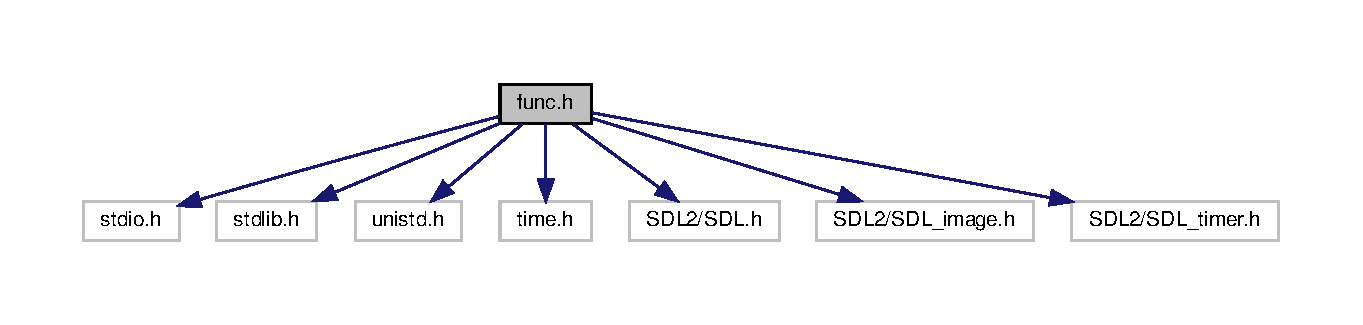
\includegraphics[width=350pt]{func_8h__incl}
\end{center}
\end{figure}
This graph shows which files directly or indirectly include this file\+:
\nopagebreak
\begin{figure}[H]
\begin{center}
\leavevmode
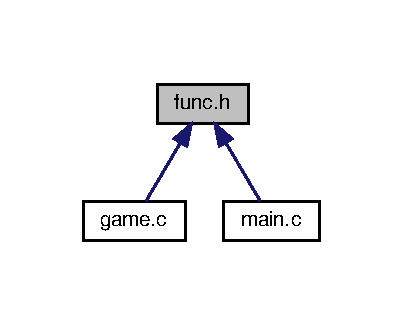
\includegraphics[width=194pt]{func_8h__dep__incl}
\end{center}
\end{figure}
\subsection*{Macros}
\begin{DoxyCompactItemize}
\item 
\#define \hyperlink{func_8h_a17e3571785d83b356acc573fc7fbdaea}{heigh}~30
\item 
\#define \hyperlink{func_8h_a667b04d7fb6ef46db4da4af554c5b6f7}{width}~80
\end{DoxyCompactItemize}
\subsection*{Functions}
\begin{DoxyCompactItemize}
\item 
void \hyperlink{func_8h_a913873cf89f388d70a28de0b77d68884}{generate} ()
\begin{DoxyCompactList}\small\item\em Generates the table based on the selected capacity level. \end{DoxyCompactList}\item 
void \hyperlink{func_8h_a197169219893d60d8a36183dbf608f34}{display} (char world\mbox{[}\hyperlink{func_8h_a667b04d7fb6ef46db4da4af554c5b6f7}{width}\mbox{]}\mbox{[}\hyperlink{func_8h_a17e3571785d83b356acc573fc7fbdaea}{heigh}\mbox{]})
\item 
void \hyperlink{func_8h_a05759d69554b6fd2f453d6ee11a7816b}{rules} (int b, int c, char table1\mbox{[}\hyperlink{func_8h_a667b04d7fb6ef46db4da4af554c5b6f7}{width}\mbox{]}\mbox{[}\hyperlink{func_8h_a17e3571785d83b356acc573fc7fbdaea}{heigh}\mbox{]}, char tableN\mbox{[}\hyperlink{func_8h_a667b04d7fb6ef46db4da4af554c5b6f7}{width}\mbox{]}\mbox{[}\hyperlink{func_8h_a17e3571785d83b356acc573fc7fbdaea}{heigh}\mbox{]})
\end{DoxyCompactItemize}
\subsection*{Variables}
\begin{DoxyCompactItemize}
\item 
int \hyperlink{func_8h_adbe66a087ac3fd4a5b0566f64ca2d12b}{capacity}
\item 
char \hyperlink{func_8h_a8bde76600e70fb4f2d289ab5a27c1d39}{table\+\_\+t} \mbox{[}\hyperlink{func_8h_a667b04d7fb6ef46db4da4af554c5b6f7}{width}\mbox{]}\mbox{[}\hyperlink{func_8h_a17e3571785d83b356acc573fc7fbdaea}{heigh}\mbox{]}
\item 
char \hyperlink{func_8h_af978b09d0f2fdfc6fd0f6f4006c71fcb}{table\+\_\+N} \mbox{[}\hyperlink{func_8h_a667b04d7fb6ef46db4da4af554c5b6f7}{width}\mbox{]}\mbox{[}\hyperlink{func_8h_a17e3571785d83b356acc573fc7fbdaea}{heigh}\mbox{]}
\end{DoxyCompactItemize}


\subsection{Macro Definition Documentation}
\mbox{\Hypertarget{func_8h_a17e3571785d83b356acc573fc7fbdaea}\label{func_8h_a17e3571785d83b356acc573fc7fbdaea}} 
\index{func.\+h@{func.\+h}!heigh@{heigh}}
\index{heigh@{heigh}!func.\+h@{func.\+h}}
\subsubsection{\texorpdfstring{heigh}{heigh}}
{\footnotesize\ttfamily \#define heigh~30}

\mbox{\Hypertarget{func_8h_a667b04d7fb6ef46db4da4af554c5b6f7}\label{func_8h_a667b04d7fb6ef46db4da4af554c5b6f7}} 
\index{func.\+h@{func.\+h}!width@{width}}
\index{width@{width}!func.\+h@{func.\+h}}
\subsubsection{\texorpdfstring{width}{width}}
{\footnotesize\ttfamily \#define width~80}



\subsection{Function Documentation}
\mbox{\Hypertarget{func_8h_a197169219893d60d8a36183dbf608f34}\label{func_8h_a197169219893d60d8a36183dbf608f34}} 
\index{func.\+h@{func.\+h}!display@{display}}
\index{display@{display}!func.\+h@{func.\+h}}
\subsubsection{\texorpdfstring{display()}{display()}}
{\footnotesize\ttfamily void display (\begin{DoxyParamCaption}\item[{char}]{world\mbox{[}width\mbox{]}\mbox{[}heigh\mbox{]} }\end{DoxyParamCaption})}


\begin{DoxyCode}
32                                       \{
33 
34     \textcolor{keywordflow}{for} (\textcolor{keywordtype}{int} j = 0; j < \hyperlink{func_8h_a17e3571785d83b356acc573fc7fbdaea}{heigh}; j++)\{
35         \textcolor{keywordflow}{for}(\textcolor{keywordtype}{int} i = 0 ;i < \hyperlink{func_8h_a667b04d7fb6ef46db4da4af554c5b6f7}{width}; i++)\{
36             printf(\textcolor{stringliteral}{"\(\backslash\)033[31m%c"}, world[i][j]);                  
37         \}
38         printf(\textcolor{stringliteral}{"\(\backslash\)n"});
39     \}
40 \}
\end{DoxyCode}
Here is the caller graph for this function\+:
\nopagebreak
\begin{figure}[H]
\begin{center}
\leavevmode
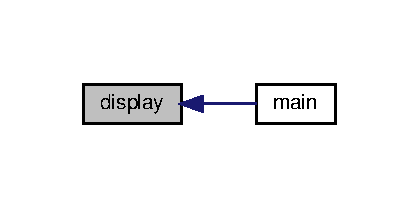
\includegraphics[width=201pt]{func_8h_a197169219893d60d8a36183dbf608f34_icgraph}
\end{center}
\end{figure}
\mbox{\Hypertarget{func_8h_a913873cf89f388d70a28de0b77d68884}\label{func_8h_a913873cf89f388d70a28de0b77d68884}} 
\index{func.\+h@{func.\+h}!generate@{generate}}
\index{generate@{generate}!func.\+h@{func.\+h}}
\subsubsection{\texorpdfstring{generate()}{generate()}}
{\footnotesize\ttfamily generate (\begin{DoxyParamCaption}{ }\end{DoxyParamCaption})}



Generates the table based on the selected capacity level. 


\begin{DoxyCode}
14                \{
15     \textcolor{keywordtype}{int} life;
16     \textcolor{keywordflow}{for} (\textcolor{keywordtype}{int} j=0;j<\hyperlink{func_8h_a17e3571785d83b356acc573fc7fbdaea}{heigh};j++)\{
17         \textcolor{keywordflow}{for}(\textcolor{keywordtype}{int} i=0;i<\hyperlink{func_8h_a667b04d7fb6ef46db4da4af554c5b6f7}{width};i++)\{
18             life=(rand()%9);
19             \textcolor{keywordflow}{if} (life<\hyperlink{func_8h_adbe66a087ac3fd4a5b0566f64ca2d12b}{capacity}) \{
20                 \hyperlink{func_8h_a8bde76600e70fb4f2d289ab5a27c1d39}{table\_t}[i][j]=\textcolor{charliteral}{'0'};
21             \}
22             \textcolor{keywordflow}{else}\{ \hyperlink{func_8h_a8bde76600e70fb4f2d289ab5a27c1d39}{table\_t}[i][j]=\textcolor{charliteral}{' '};
23             \}
24         \}
25     \}
26 \}
\end{DoxyCode}
Here is the caller graph for this function\+:
\nopagebreak
\begin{figure}[H]
\begin{center}
\leavevmode
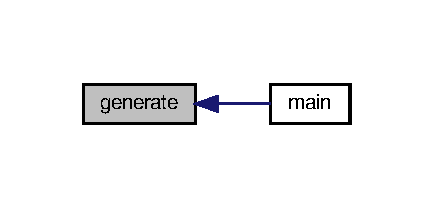
\includegraphics[width=208pt]{func_8h_a913873cf89f388d70a28de0b77d68884_icgraph}
\end{center}
\end{figure}
\mbox{\Hypertarget{func_8h_a05759d69554b6fd2f453d6ee11a7816b}\label{func_8h_a05759d69554b6fd2f453d6ee11a7816b}} 
\index{func.\+h@{func.\+h}!rules@{rules}}
\index{rules@{rules}!func.\+h@{func.\+h}}
\subsubsection{\texorpdfstring{rules()}{rules()}}
{\footnotesize\ttfamily void rules (\begin{DoxyParamCaption}\item[{int}]{b,  }\item[{int}]{c,  }\item[{char}]{table1\mbox{[}width\mbox{]}\mbox{[}heigh\mbox{]},  }\item[{char}]{tableN\mbox{[}width\mbox{]}\mbox{[}heigh\mbox{]} }\end{DoxyParamCaption})}

if cell is alive

Due to the rules

Not generating properly with iy
\begin{DoxyCode}
42                                                                               \{ \textcolor{comment}{// Checks how many living
       neighbors this tile currently has.}
43     \textcolor{keywordtype}{int} neighbors = 0;
44     \textcolor{keywordflow}{for} (\textcolor{keywordtype}{int} i = -1; i <= 1; i++) \{
45         \textcolor{keywordflow}{for} (\textcolor{keywordtype}{int} j = -1; j <= 1; j++) \{
46             \textcolor{keywordflow}{if} ((i == 0 && j == 0) || b + i >= \hyperlink{func_8h_a667b04d7fb6ef46db4da4af554c5b6f7}{width} || b + i < 0 || c + j >= 
      \hyperlink{func_8h_a17e3571785d83b356acc573fc7fbdaea}{heigh}  || c + j < 0) \{ \textcolor{comment}{//either in current cell or neightb.}
47                 \textcolor{keywordflow}{continue};   
48             \}
52             \textcolor{keywordflow}{if} (table1[b + i][c + j] == \textcolor{charliteral}{'0'})\{
53                 neighbors++;
54             \}
55         \} 
56     \}
57     
61     \textcolor{keywordflow}{if} (neighbors == 3 || (neighbors == 2 && table1[b][c] == \textcolor{charliteral}{'0'})) \{ \textcolor{comment}{//Any live cell with two or three live
       neighbors survives.}
62         tableN[b][c] = \textcolor{charliteral}{'0'};
63     \} \textcolor{keywordflow}{else} \{
64         tableN[b][c] = \textcolor{charliteral}{' '};
65     \}
69     \textcolor{comment}{//    if (neighbors == 3 || table1[b][c] == ' ') \{//Any dead cell with three live neighbors becomes a
       live cell.}
70     \textcolor{comment}{//  tableN[b][c] = '0';}
71     \textcolor{comment}{// \} else \{}
72     \textcolor{comment}{//  tableN[b][c] = ' ';}
73     \textcolor{comment}{// \}}
74 \}
\end{DoxyCode}
Here is the caller graph for this function\+:
\nopagebreak
\begin{figure}[H]
\begin{center}
\leavevmode
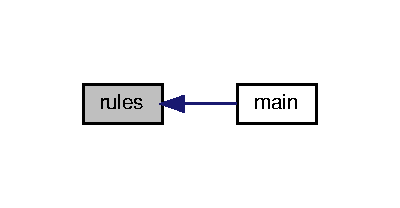
\includegraphics[width=192pt]{func_8h_a05759d69554b6fd2f453d6ee11a7816b_icgraph}
\end{center}
\end{figure}


\subsection{Variable Documentation}
\mbox{\Hypertarget{func_8h_adbe66a087ac3fd4a5b0566f64ca2d12b}\label{func_8h_adbe66a087ac3fd4a5b0566f64ca2d12b}} 
\index{func.\+h@{func.\+h}!capacity@{capacity}}
\index{capacity@{capacity}!func.\+h@{func.\+h}}
\subsubsection{\texorpdfstring{capacity}{capacity}}
{\footnotesize\ttfamily int capacity}

\mbox{\Hypertarget{func_8h_af978b09d0f2fdfc6fd0f6f4006c71fcb}\label{func_8h_af978b09d0f2fdfc6fd0f6f4006c71fcb}} 
\index{func.\+h@{func.\+h}!table\+\_\+N@{table\+\_\+N}}
\index{table\+\_\+N@{table\+\_\+N}!func.\+h@{func.\+h}}
\subsubsection{\texorpdfstring{table\+\_\+N}{table\_N}}
{\footnotesize\ttfamily char table\+\_\+N\mbox{[}\hyperlink{func_8h_a667b04d7fb6ef46db4da4af554c5b6f7}{width}\mbox{]}\mbox{[}\hyperlink{func_8h_a17e3571785d83b356acc573fc7fbdaea}{heigh}\mbox{]}}

\mbox{\Hypertarget{func_8h_a8bde76600e70fb4f2d289ab5a27c1d39}\label{func_8h_a8bde76600e70fb4f2d289ab5a27c1d39}} 
\index{func.\+h@{func.\+h}!table\+\_\+t@{table\+\_\+t}}
\index{table\+\_\+t@{table\+\_\+t}!func.\+h@{func.\+h}}
\subsubsection{\texorpdfstring{table\+\_\+t}{table\_t}}
{\footnotesize\ttfamily char table\+\_\+t\mbox{[}\hyperlink{func_8h_a667b04d7fb6ef46db4da4af554c5b6f7}{width}\mbox{]}\mbox{[}\hyperlink{func_8h_a17e3571785d83b356acc573fc7fbdaea}{heigh}\mbox{]}}


\hypertarget{game_8c}{}\section{game.\+c File Reference}
\label{game_8c}\index{game.\+c@{game.\+c}}


game  Source code of Conway\textquotesingle{}s Game Of Life  


{\ttfamily \#include \char`\"{}func.\+h\char`\"{}}\newline
{\ttfamily \#include $<$S\+D\+L2/\+S\+D\+L.\+h$>$}\newline
Include dependency graph for game.\+c\+:
\nopagebreak
\begin{figure}[H]
\begin{center}
\leavevmode
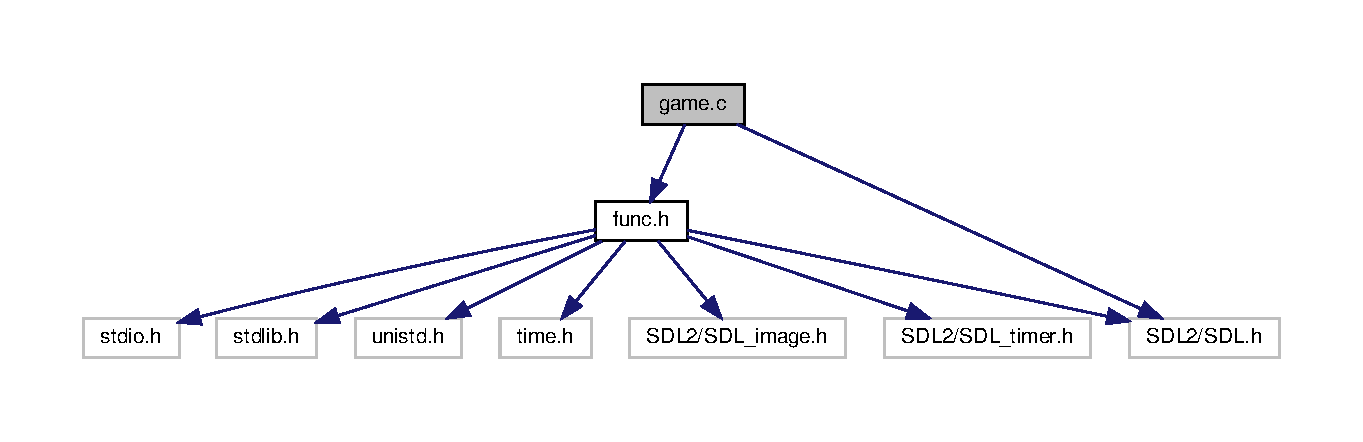
\includegraphics[width=350pt]{game_8c__incl}
\end{center}
\end{figure}
\subsection*{Functions}
\begin{DoxyCompactItemize}
\item 
void \hyperlink{game_8c_a3c01631a4116e8810c6c1021d7110ab7}{generate} ()
\begin{DoxyCompactList}\small\item\em Generates the table based on the selected capacity level. \end{DoxyCompactList}\item 
void \hyperlink{game_8c_a197169219893d60d8a36183dbf608f34}{display} (char world\mbox{[}\hyperlink{func_8h_a667b04d7fb6ef46db4da4af554c5b6f7}{width}\mbox{]}\mbox{[}\hyperlink{func_8h_a17e3571785d83b356acc573fc7fbdaea}{heigh}\mbox{]})
\item 
void \hyperlink{game_8c_a05759d69554b6fd2f453d6ee11a7816b}{rules} (int b, int c, char table1\mbox{[}\hyperlink{func_8h_a667b04d7fb6ef46db4da4af554c5b6f7}{width}\mbox{]}\mbox{[}\hyperlink{func_8h_a17e3571785d83b356acc573fc7fbdaea}{heigh}\mbox{]}, char tableN\mbox{[}\hyperlink{func_8h_a667b04d7fb6ef46db4da4af554c5b6f7}{width}\mbox{]}\mbox{[}\hyperlink{func_8h_a17e3571785d83b356acc573fc7fbdaea}{heigh}\mbox{]})
\end{DoxyCompactItemize}


\subsection{Detailed Description}
game  Source code of Conway\textquotesingle{}s Game Of Life 


\begin{DoxyCodeInclude}
\end{DoxyCodeInclude}
 

\subsection{Function Documentation}
\mbox{\Hypertarget{game_8c_a197169219893d60d8a36183dbf608f34}\label{game_8c_a197169219893d60d8a36183dbf608f34}} 
\index{game.\+c@{game.\+c}!display@{display}}
\index{display@{display}!game.\+c@{game.\+c}}
\subsubsection{\texorpdfstring{display()}{display()}}
{\footnotesize\ttfamily void display (\begin{DoxyParamCaption}\item[{char}]{world\mbox{[}width\mbox{]}\mbox{[}heigh\mbox{]} }\end{DoxyParamCaption})}


\begin{DoxyCode}
32                                       \{
33 
34     \textcolor{keywordflow}{for} (\textcolor{keywordtype}{int} j = 0; j < \hyperlink{func_8h_a17e3571785d83b356acc573fc7fbdaea}{heigh}; j++)\{
35         \textcolor{keywordflow}{for}(\textcolor{keywordtype}{int} i = 0 ;i < \hyperlink{func_8h_a667b04d7fb6ef46db4da4af554c5b6f7}{width}; i++)\{
36             printf(\textcolor{stringliteral}{"\(\backslash\)033[31m%c"}, world[i][j]);                  
37         \}
38         printf(\textcolor{stringliteral}{"\(\backslash\)n"});
39     \}
40 \}
\end{DoxyCode}
Here is the caller graph for this function\+:
\nopagebreak
\begin{figure}[H]
\begin{center}
\leavevmode
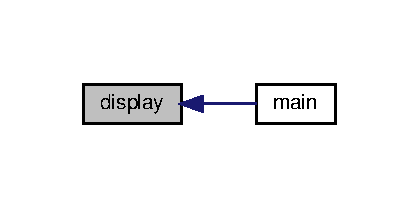
\includegraphics[width=201pt]{game_8c_a197169219893d60d8a36183dbf608f34_icgraph}
\end{center}
\end{figure}
\mbox{\Hypertarget{game_8c_a3c01631a4116e8810c6c1021d7110ab7}\label{game_8c_a3c01631a4116e8810c6c1021d7110ab7}} 
\index{game.\+c@{game.\+c}!generate@{generate}}
\index{generate@{generate}!game.\+c@{game.\+c}}
\subsubsection{\texorpdfstring{generate()}{generate()}}
{\footnotesize\ttfamily void generate (\begin{DoxyParamCaption}{ }\end{DoxyParamCaption})}



Generates the table based on the selected capacity level. 


\begin{DoxyCode}
14                \{
15     \textcolor{keywordtype}{int} life;
16     \textcolor{keywordflow}{for} (\textcolor{keywordtype}{int} j=0;j<\hyperlink{func_8h_a17e3571785d83b356acc573fc7fbdaea}{heigh};j++)\{
17         \textcolor{keywordflow}{for}(\textcolor{keywordtype}{int} i=0;i<\hyperlink{func_8h_a667b04d7fb6ef46db4da4af554c5b6f7}{width};i++)\{
18             life=(rand()%9);
19             \textcolor{keywordflow}{if} (life<\hyperlink{func_8h_adbe66a087ac3fd4a5b0566f64ca2d12b}{capacity}) \{
20                 \hyperlink{func_8h_a8bde76600e70fb4f2d289ab5a27c1d39}{table\_t}[i][j]=\textcolor{charliteral}{'0'};
21             \}
22             \textcolor{keywordflow}{else}\{ \hyperlink{func_8h_a8bde76600e70fb4f2d289ab5a27c1d39}{table\_t}[i][j]=\textcolor{charliteral}{' '};
23             \}
24         \}
25     \}
26 \}
\end{DoxyCode}
Here is the caller graph for this function\+:
\nopagebreak
\begin{figure}[H]
\begin{center}
\leavevmode
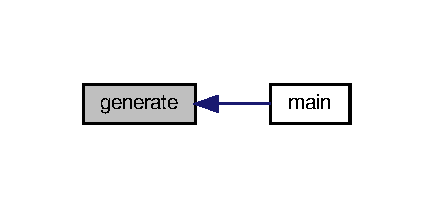
\includegraphics[width=208pt]{game_8c_a3c01631a4116e8810c6c1021d7110ab7_icgraph}
\end{center}
\end{figure}
\mbox{\Hypertarget{game_8c_a05759d69554b6fd2f453d6ee11a7816b}\label{game_8c_a05759d69554b6fd2f453d6ee11a7816b}} 
\index{game.\+c@{game.\+c}!rules@{rules}}
\index{rules@{rules}!game.\+c@{game.\+c}}
\subsubsection{\texorpdfstring{rules()}{rules()}}
{\footnotesize\ttfamily void rules (\begin{DoxyParamCaption}\item[{int}]{b,  }\item[{int}]{c,  }\item[{char}]{table1\mbox{[}width\mbox{]}\mbox{[}heigh\mbox{]},  }\item[{char}]{tableN\mbox{[}width\mbox{]}\mbox{[}heigh\mbox{]} }\end{DoxyParamCaption})}

if cell is alive

Due to the rules

Not generating properly with iy
\begin{DoxyCode}
42                                                                               \{ \textcolor{comment}{// Checks how many living
       neighbors this tile currently has.}
43     \textcolor{keywordtype}{int} neighbors = 0;
44     \textcolor{keywordflow}{for} (\textcolor{keywordtype}{int} i = -1; i <= 1; i++) \{
45         \textcolor{keywordflow}{for} (\textcolor{keywordtype}{int} j = -1; j <= 1; j++) \{
46             \textcolor{keywordflow}{if} ((i == 0 && j == 0) || b + i >= \hyperlink{func_8h_a667b04d7fb6ef46db4da4af554c5b6f7}{width} || b + i < 0 || c + j >= 
      \hyperlink{func_8h_a17e3571785d83b356acc573fc7fbdaea}{heigh}  || c + j < 0) \{ \textcolor{comment}{//either in current cell or neightb.}
47                 \textcolor{keywordflow}{continue};   
48             \}
52             \textcolor{keywordflow}{if} (table1[b + i][c + j] == \textcolor{charliteral}{'0'})\{
53                 neighbors++;
54             \}
55         \} 
56     \}
57     
61     \textcolor{keywordflow}{if} (neighbors == 3 || (neighbors == 2 && table1[b][c] == \textcolor{charliteral}{'0'})) \{ \textcolor{comment}{//Any live cell with two or three live
       neighbors survives.}
62         tableN[b][c] = \textcolor{charliteral}{'0'};
63     \} \textcolor{keywordflow}{else} \{
64         tableN[b][c] = \textcolor{charliteral}{' '};
65     \}
69     \textcolor{comment}{//    if (neighbors == 3 || table1[b][c] == ' ') \{//Any dead cell with three live neighbors becomes a
       live cell.}
70     \textcolor{comment}{//  tableN[b][c] = '0';}
71     \textcolor{comment}{// \} else \{}
72     \textcolor{comment}{//  tableN[b][c] = ' ';}
73     \textcolor{comment}{// \}}
74 \}
\end{DoxyCode}
Here is the caller graph for this function\+:
\nopagebreak
\begin{figure}[H]
\begin{center}
\leavevmode
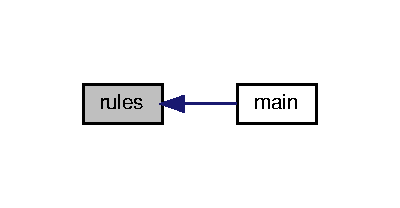
\includegraphics[width=192pt]{game_8c_a05759d69554b6fd2f453d6ee11a7816b_icgraph}
\end{center}
\end{figure}

\hypertarget{main_8c}{}\section{main.\+c File Reference}
\label{main_8c}\index{main.\+c@{main.\+c}}


main function  Main file of Conway\textquotesingle{}s Game Of Life project  


{\ttfamily \#include $<$stdio.\+h$>$}\newline
{\ttfamily \#include $<$stdlib.\+h$>$}\newline
{\ttfamily \#include $<$unistd.\+h$>$}\newline
{\ttfamily \#include $<$S\+D\+L2/\+S\+D\+L.\+h$>$}\newline
{\ttfamily \#include \char`\"{}func.\+h\char`\"{}}\newline
Include dependency graph for main.\+c\+:
\nopagebreak
\begin{figure}[H]
\begin{center}
\leavevmode
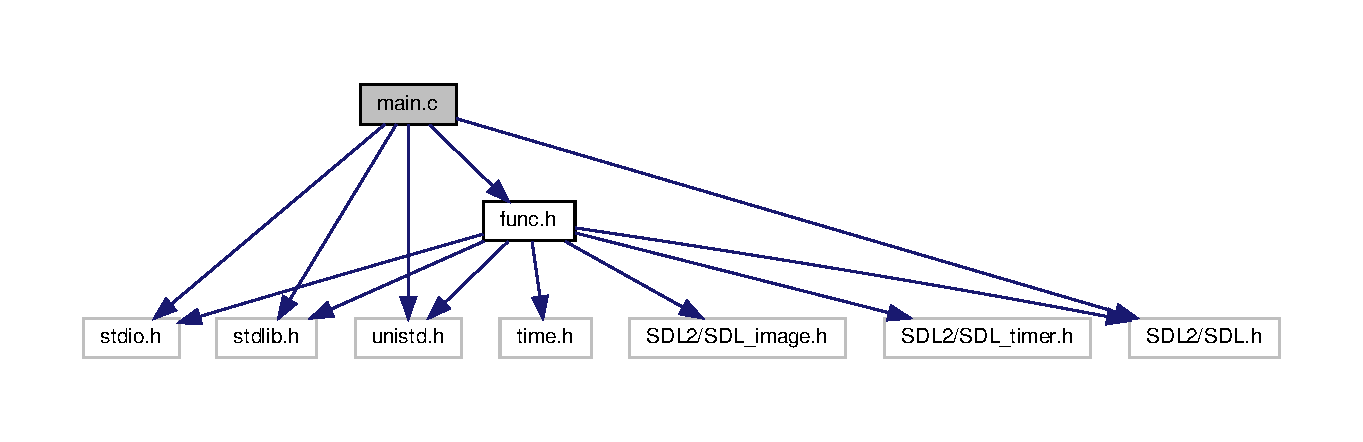
\includegraphics[width=350pt]{main_8c__incl}
\end{center}
\end{figure}
\subsection*{Functions}
\begin{DoxyCompactItemize}
\item 
int \hyperlink{main_8c_a51af30a60f9f02777c6396b8247e356f}{main} ()
\begin{DoxyCompactList}\small\item\em generating tables and creating the game due to random 7 type of position which the user select \end{DoxyCompactList}\end{DoxyCompactItemize}


\subsection{Detailed Description}
main function  Main file of Conway\textquotesingle{}s Game Of Life project 


\begin{DoxyCodeInclude}
\end{DoxyCodeInclude}
 

\subsection{Function Documentation}
\mbox{\Hypertarget{main_8c_a51af30a60f9f02777c6396b8247e356f}\label{main_8c_a51af30a60f9f02777c6396b8247e356f}} 
\index{main.\+c@{main.\+c}!main@{main}}
\index{main@{main}!main.\+c@{main.\+c}}
\subsubsection{\texorpdfstring{main()}{main()}}
{\footnotesize\ttfamily main (\begin{DoxyParamCaption}{ }\end{DoxyParamCaption})}



generating tables and creating the game due to random 7 type of position which the user select 

Taking the capacity \begin{DoxyWarning}{Warning}
Only range of \mbox{[}1;7\mbox{]} acceptable, otherwise it\textquotesingle{}ll ask again untill get the integer in that range
\end{DoxyWarning}
Generates new table

\begin{DoxyWarning}{Warning}
draft S\+DL
\end{DoxyWarning}
Displays the datas in the t and t+1 tables separately

\begin{DoxyWarning}{Warning}
draft S\+DL

for compiling with S\+DL\+: gcc \hyperlink{game_8c}{game.\+c} \hyperlink{main_8c}{main.\+c} {\ttfamily sdl2-\/config -\/-\/cflags -\/-\/libs} -\/l\+S\+D\+L2 -\/l\+S\+D\+L2\+\_\+mixer -\/l\+S\+D\+L2\+\_\+image -\/l\+S\+D\+L2\+\_\+ttfgcc \hyperlink{game_8c}{game.\+c} \hyperlink{main_8c}{main.\+c} {\ttfamily sdl2-\/config -\/-\/cflags -\/-\/libs} -\/l\+S\+D\+L2 -\/l\+S\+D\+L2\+\_\+mixer -\/l\+S\+D\+L2\+\_\+image -\/l\+S\+D\+L2\+\_\+ttf
\end{DoxyWarning}

\begin{DoxyCode}
18           \{
19 \textcolor{comment}{// unsigned char copy[width * heigh];}
20 \textcolor{comment}{//unsigned char pixels[width * heigh * 4];}
21     \hyperlink{func_8h_adbe66a087ac3fd4a5b0566f64ca2d12b}{capacity} = 0;
22     \textcolor{keywordtype}{char} start;
23     srand(time(NULL));
24 
29     printf(\textcolor{stringliteral}{"Please, choose the starting capacity level in [1; 7] range:\(\backslash\)n"});
30     \textcolor{keywordtype}{char} buffer[80] = \textcolor{stringliteral}{""};
31     \textcolor{keywordflow}{for}(\textcolor{keywordtype}{int} i=0; i<7; i++)\{
32         fgets(buffer, \textcolor{keyword}{sizeof}(buffer), stdin);
33         \textcolor{keywordflow}{if} (sscanf(buffer, \textcolor{stringliteral}{"%d"}, &\hyperlink{func_8h_adbe66a087ac3fd4a5b0566f64ca2d12b}{capacity}) != 1) \{
34             \hyperlink{func_8h_adbe66a087ac3fd4a5b0566f64ca2d12b}{capacity} = 0;
35         \}
36         \textcolor{keywordflow}{if} (\hyperlink{func_8h_adbe66a087ac3fd4a5b0566f64ca2d12b}{capacity} >= 1 && \hyperlink{func_8h_adbe66a087ac3fd4a5b0566f64ca2d12b}{capacity} <= 7) \{
37             \textcolor{keywordflow}{break};
38         \}
39         printf(\textcolor{stringliteral}{"Please, choose the starting capacity level in [1; 7] range:\(\backslash\)n"});
40     \}
41     
45     \hyperlink{func_8h_a913873cf89f388d70a28de0b77d68884}{generate}();
46 
50 \textcolor{comment}{// SDL\_Init(SDL\_INIT\_VIDEO);}
51 \textcolor{comment}{// SDL\_Window *window = SDL\_CreateWindow("life", SDL\_WINDOWPOS\_UNDEFINED, SDL\_WINDOWPOS\_UNDEFINED, width,
       heigh, SDL\_WINDOW\_SHOWN);}
52 \textcolor{comment}{// SDL\_Renderer *renderer = SDL\_CreateRenderer(window, -1, SDL\_RENDERER\_ACCELERATED);}
53 \textcolor{comment}{// SDL\_Texture *texture = SDL\_CreateTexture(renderer, SDL\_PIXELFORMAT\_RGBA32, SDL\_TEXTUREACCESS\_STREAMING,
       width, heigh);}
54 \textcolor{comment}{// SDL\_Event event;}
55 \textcolor{comment}{// while (1) \{}
56 \textcolor{comment}{//     if (SDL\_PollEvent(&event)) \{}
57 \textcolor{comment}{//       if (event.type == SDL\_QUIT) \{}
58 \textcolor{comment}{//         break;}
59 \textcolor{comment}{//       \}}
60 \textcolor{comment}{//     \}}
61 
65     \hyperlink{func_8h_a197169219893d60d8a36183dbf608f34}{display}(\hyperlink{func_8h_a8bde76600e70fb4f2d289ab5a27c1d39}{table\_t}); 
66     printf(\textcolor{stringliteral}{"\(\backslash\)n\(\backslash\)n Type '1' to play the game.\(\backslash\)n Type '0' to exit.\(\backslash\)n"});
67     \textcolor{comment}{// printf("\(\backslash\)033[2J");}
68     \textcolor{keywordtype}{int} turn = 0;
69     \textcolor{keywordtype}{int} generation;
70     scanf(\textcolor{stringliteral}{"\(\backslash\)n%c"}, &start);
71     \textcolor{keywordflow}{if} (start == \textcolor{charliteral}{'1'})\{
72         \textcolor{keywordflow}{for}(generation = 0; generation < 150; generation++) \{
73             usleep(30000);
74             \textcolor{comment}{// printf("\(\backslash\)033[2J");}
75             \textcolor{keywordflow}{if} (turn == 0)\{
76                                 \textcolor{keywordflow}{for} (\textcolor{keywordtype}{int} j = 0; j < \hyperlink{func_8h_a17e3571785d83b356acc573fc7fbdaea}{heigh}; j++)\{
77                     \textcolor{keywordflow}{for} (\textcolor{keywordtype}{int} i = 0; i < \hyperlink{func_8h_a667b04d7fb6ef46db4da4af554c5b6f7}{width}; i++)\{
78                         \hyperlink{func_8h_a05759d69554b6fd2f453d6ee11a7816b}{rules}(i, j, \hyperlink{func_8h_a8bde76600e70fb4f2d289ab5a27c1d39}{table\_t}, \hyperlink{func_8h_af978b09d0f2fdfc6fd0f6f4006c71fcb}{table\_N});
79                     \}
80                 \}
81                 \hyperlink{func_8h_a197169219893d60d8a36183dbf608f34}{display}(\hyperlink{func_8h_af978b09d0f2fdfc6fd0f6f4006c71fcb}{table\_N});
82                 turn = 1;
83 
84             \} \textcolor{keywordflow}{else} \textcolor{keywordflow}{if} (turn == 1)\{
85                 \textcolor{keywordflow}{for} (\textcolor{keywordtype}{int} j = 0; j < \hyperlink{func_8h_a17e3571785d83b356acc573fc7fbdaea}{heigh}; j++)\{
86                     \textcolor{keywordflow}{for} (\textcolor{keywordtype}{int} i = 0; i < \hyperlink{func_8h_a667b04d7fb6ef46db4da4af554c5b6f7}{width}; i++)\{
87                         \hyperlink{func_8h_a05759d69554b6fd2f453d6ee11a7816b}{rules}(i, j, \hyperlink{func_8h_af978b09d0f2fdfc6fd0f6f4006c71fcb}{table\_N}, \hyperlink{func_8h_a8bde76600e70fb4f2d289ab5a27c1d39}{table\_t});
88                     \}
89                 \}
90                 \hyperlink{func_8h_a197169219893d60d8a36183dbf608f34}{display}(\hyperlink{func_8h_a8bde76600e70fb4f2d289ab5a27c1d39}{table\_t});
91                 turn = 0;
92             \}
93             usleep(30000);
94             printf(\textcolor{stringliteral}{"\(\backslash\)033[r;cH"});
95             
96         \}
97     \}
98 
102   \textcolor{comment}{//   SDL\_UpdateTexture(texture, NULL, pixels, width * 16);}
103   \textcolor{comment}{//   SDL\_SetRenderDrawColor(renderer, 0, 0, 0, SDL\_ALPHA\_OPAQUE);}
104   \textcolor{comment}{//   SDL\_RenderClear(renderer);}
105   \textcolor{comment}{//   SDL\_RenderCopy(renderer, texture, NULL, NULL);}
106   \textcolor{comment}{//   SDL\_RenderPresent(renderer);}
107   \textcolor{comment}{//   SDL\_Delay(5);}
108   \textcolor{comment}{// \}}
109   \textcolor{comment}{// SDL\_DestroyTexture(texture);}
110   \textcolor{comment}{// SDL\_DestroyRenderer(renderer);}
111   \textcolor{comment}{// SDL\_DestroyWindow(window);}
112   \textcolor{comment}{// SDL\_Quit();}
113   \textcolor{comment}{// return 0;}
118 \textcolor{comment}{}\}
\end{DoxyCode}
Here is the call graph for this function\+:
\nopagebreak
\begin{figure}[H]
\begin{center}
\leavevmode
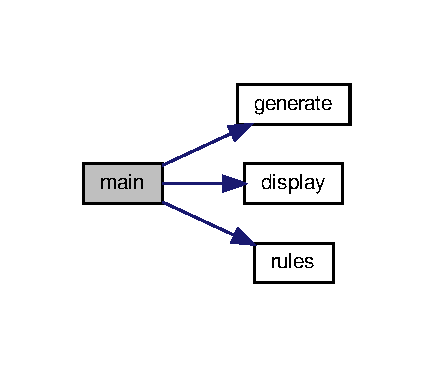
\includegraphics[width=208pt]{main_8c_a51af30a60f9f02777c6396b8247e356f_cgraph}
\end{center}
\end{figure}

%--- End generated contents ---

% Index
\backmatter
\newpage
\phantomsection
\clearemptydoublepage
\addcontentsline{toc}{chapter}{Index}
\printindex

\end{document}
